\documentclass[tikz,border=4pt]{standalone}
\usepackage{tikz}
\usepackage{pgfplots}
\usepackage{amsmath}
\pgfplotsset{compat=1.18}

\begin{document}
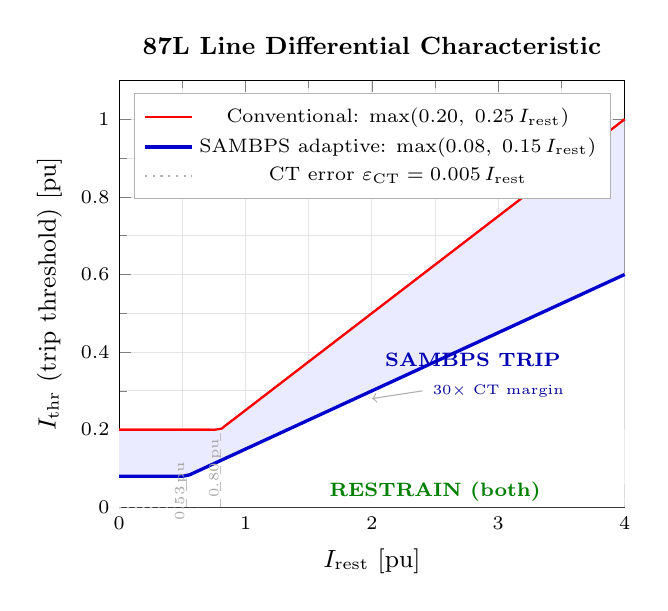
\begin{tikzpicture}
\begin{axis}[
  width=8cm, height=7cm,
  xlabel={$I_{\rm rest}$ [pu]},
  ylabel={$I_{\rm thr}$ (trip threshold) [pu]},
  xmin=0, xmax=4.0,
  ymin=0, ymax=1.1,
  grid=both,
  grid style={gray!20, line width=0.3pt},
  minor tick num=1,
  tick label style={font=\scriptsize},
  label style={font=\small},
  legend style={font=\scriptsize, at={(0.03,0.97)}, anchor=north west,
                fill=white, draw=black!30, inner sep=3pt},
  title style={font=\small\bfseries},
  title={87L Line Differential Characteristic},
  clip=false,
]

%% ── IBR fault current failure zone (shaded, behind everything) ──────────────
%% Conventional relay fails when I_diff in [0.06, 0.20] pu (below threshold)
\addplot[fill=red!12, draw=none, forget plot]
  coordinates {(0,0.06)(4.0,0.06)(4.0,0.20)(0,0.20)(0,0.06)};
\node[font=\tiny, red!70!black, align=center] at (axis cs:3.1,0.13)
  {IBR fault zone\\(conv.\ fails)};

%% ── Conventional relay: fixed slope + fixed floor ───────────────────────────
\addplot[red, thick, domain=0:4.0, samples=80]
  { max(0.20, 0.25*x) };
\addlegendentry{Conventional: $\max(0.20,\; 0.25\,I_{\rm rest})$}

%% ── SAMBPS adaptive threshold ───────────────────────────────────────────────
\addplot[blue!80!black, very thick, domain=0:4.0, samples=80]
  { max(0.08, 0.15*x) };
\addlegendentry{SAMBPS adaptive: $\max(0.08,\; 0.15\,I_{\rm rest})$}

%% ── CT error reference curve ────────────────────────────────────────────────
\addplot[gray!60, dotted, thick, domain=0:4.0]
  { 0.005*x };
\addlegendentry{CT error $\varepsilon_{\rm CT}=0.005\,I_{\rm rest}$}

%% ── SAMBPS recovery fill (between adaptive threshold and conventional) ──────
\addplot[blue!8, fill=blue!8, draw=none, forget plot, domain=0:4.0]
  { max(0.20, 0.25*x) } \closedcycle;
\addplot[white, fill=white, draw=none, forget plot, domain=0:4.0]
  { max(0.08, 0.15*x) } \closedcycle;

%% ── Redraw curves on top of fills ───────────────────────────────────────────
\addplot[red, thick, domain=0:4.0, samples=80, forget plot]
  { max(0.20, 0.25*x) };
\addplot[blue!80!black, very thick, domain=0:4.0, samples=80, forget plot]
  { max(0.08, 0.15*x) };

%% ── Breakpoints ─────────────────────────────────────────────────────────────
%% Conventional knee: I_rest = 0.20/0.25 = 0.80
\draw[dashed, gray!50, thin] (axis cs:0.80,0) -- (axis cs:0.80,0.20);
\node[font=\tiny, gray!70, rotate=90] at (axis cs:0.76,0.10) {$0.80$\,pu};

%% SAMBPS knee: I_rest = 0.08/0.15 = 0.53
\draw[dashed, gray!50, thin] (axis cs:0.533,0) -- (axis cs:0.533,0.08);
\node[font=\tiny, gray!70, rotate=90] at (axis cs:0.49,0.04) {$0.53$\,pu};

%% ── Region labels ────────────────────────────────────────────────────────────
\node[font=\scriptsize\bfseries, red!70!black]
  at (axis cs:2.5,0.85)   {TRIP (both)};
\node[font=\scriptsize\bfseries, blue!70!black]
  at (axis cs:2.8,0.38)   {SAMBPS TRIP};
\node[font=\scriptsize\bfseries, green!50!black]
  at (axis cs:2.5,0.04)   {RESTRAIN (both)};

%% ── 30x margin annotation ────────────────────────────────────────────────────
\draw[->, gray!60, thin]
  (axis cs:2.4,0.30) -- (axis cs:2.0,0.28);
\node[font=\tiny, blue!60!black]
  at (axis cs:3.0,0.30) {$30\times$ CT margin};

\end{axis}
\end{tikzpicture}
\end{document}
